\section{Présentation}


\begin{frame}
	\begin{center}
		\textbf{Alice \textsc{Dinsenmeyer}}\\
		\footnotesize{Doctorante (1\textsuperscript{ère} année)\\[0.5cm]
		\textit{alice.dinsenmeyer@insa-lyon.fr\\
		1\textsuperscript{er} étage, Bât. J. Jacquard}}
		\vfill
		\normalsize
		Licence et master acoustique du Mans (2011-2016)\\[0.3cm]
		- Ondes~~~~~- Traitement du signal~~~~~- Méthodes numériques\\
		- Imagerie US~~~~- Psychoacoustique	
	\end{center}


	

%	\begin{itemize}
%		\item 2011 -- 2014 : Licence en acoustique, Université du Maine, Le Mans %Bachelor of science in acoustics
%		\item 2014 --2016 : Master recherche en acoustique, Université du Maine, Le Mans %Master of science in acoustics
%		\begin{columns}
%			\hspace{2cm}\column{0.5\textwidth}
%			\begin{itemize}
%				\item[-] Ondes dans les solides et les fluides
%				\item[-] Imagerie ultrasonore
%				\item[-] Psychoacoustique
%			\end{itemize}
%			\column{0.5\textwidth}
%			\begin{itemize}
%				\item[-] Traitement du signal
%				\item[-] Informatique scientifique
%			\end{itemize}
%		\end{columns}
%	\end{itemize}
\end{frame}

\section{Sujet de thèse}


\begin{frame}
	\centering
	\textbf{ Méthodes inverses par approche bayésienne \\pour l'identification de sources aéroacoustique}\\
	\footnotesize{depuis juillet 2017}\\[0.5cm]
	Direction : Jérôme Antoni (LVA), Chritophe Bailly (LMFA), Quentin Leclère (LVA)\\[0.5cm]
	Financements : CeLyA + INSAVALOR (projet européen \textbf{AD}vanced \textbf{A}eroacoustic \textbf{P}rocessing \textbf{T}echniques, ADAPT)

	Collaborations : LVA, LMFA, MicrodB, PSA3, Airbus
\end{frame}


\begin{frame}{Contexte}
		\begin{wrapfigure}{r}{3cm}
			\centering
			\vspace{-0.9cm}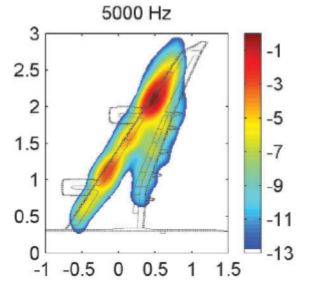
\includegraphics[width=4cm]{img/bf_sijtsma.png}\\
			\scriptsize{\itshape Beamforming, M=0.17,\\Sijtsma 2007}
			\vspace{-3cm}
		\end{wrapfigure}~
		\begin{itemize}
			\item Réduction du bruit des avions  : \\ aérodynamique et turbomachines\\   (conception et validation)\\~\\
			\item Fluctuations de pressions\\ $\hookrightarrow$ caractérisation acoustique\\~\\
			\item Sources aéroacoustiques : 
				\begin{itemize}
					\item[-] parcimonieuses spatialement,
					\item[-]  large bande fréquentielle (domaine de l'audible)
					\item[-]  mesures empreintes de bruit aérodynamique (en vol et en soufflerie)
				\end{itemize}~\\
			\item Méthodes actuelles : formation de voies \& déconvolution
				\begin{itemize}
					\item[-]  Avantages : flexible, simple et rapide
					\item[-]  Limites : connaissance du modèle de sources, sources corrélées, niveaux
				\end{itemize}
		\end{itemize}
	
\end{frame}


\begin{frame}{Axes de la thèse}
	\begin{enumerate}
		\item Débruitage des mesures : \\
			\begin{itemize}
				\item Approche bayésienne
				\item Connaissances a priori : modèles analytiques/numériques + autres données expérimentales
				\item Qualité ?
			\end{itemize}~\\
		\item Localisation des sources : approche bayésienne
			\begin{itemize}
				\item Contraindre l'inversion : physique des sources
				\item Critère de qualité ? (qualitatif et quantitatif)
				\item Méthodes numériques
			\end{itemize}
	\end{enumerate}
\end{frame}


\begin{frame}{Imagerie US vs localisation de sources}
	\begin{itemize}
		\item<1-> Localisation de sources acoustique
		\begin{figure}
			
\includegraphics[width = 6cm]{./img/pd_dir_inv/ac.png}
		\end{figure}~\\
		\item<2-> Imagerie par ultrasons
		\begin{figure}
			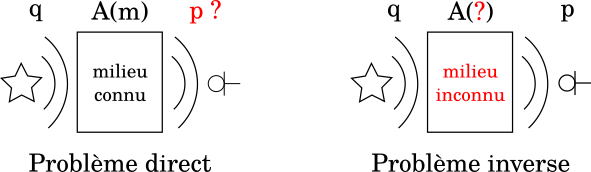
\includegraphics[width = 6cm]{./img/pd_dir_inv/us.png}
		\end{figure}
	\end{itemize}
	
\end{frame}

